\usetikzlibrary{patterns}
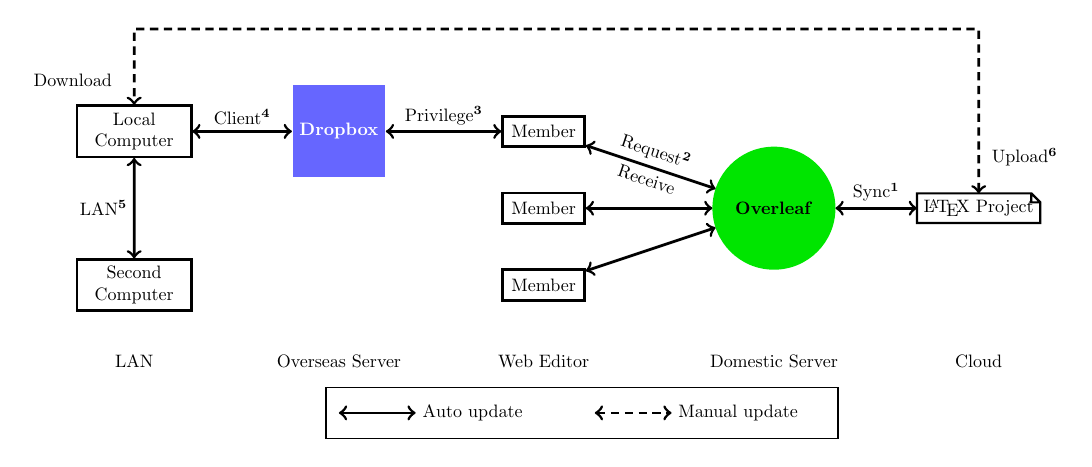
\begin{tikzpicture}[line width=1pt,scale=0.65, every node/.style={scale=0.65}] %缩放

\tikzstyle{bordered} = [circle,outer sep=0,inner sep=10,minimum size=10,fill=green!90!black];
\tikzstyle{boldarrow}=[<->,line width=1pt];

\makeatletter
      \pgfdeclareshape{document}{
      \inheritsavedanchors[from=rectangle] % this is nearly a rectangle
      \inheritanchorborder[from=rectangle]
      \inheritanchor[from=rectangle]{center}
      \inheritanchor[from=rectangle]{north}
      \inheritanchor[from=rectangle]{south}
      \inheritanchor[from=rectangle]{west}
      \inheritanchor[from=rectangle]{east}
      % ... and possibly more
      \backgroundpath{% this is new
      % store lower right in xa/ya and upper right in xb/yb
      \southwest \pgf@xa=\pgf@x \pgf@ya=\pgf@y
      \northeast \pgf@xb=\pgf@x \pgf@yb=\pgf@y
      % compute corner of ``flipped page''
      \pgf@xc=\pgf@xb \advance\pgf@xc by-5pt % this should be a parameter
      \pgf@yc=\pgf@yb \advance\pgf@yc by-5pt
      % construct main path
      \pgfpathmoveto{\pgfpoint{\pgf@xa}{\pgf@ya}}
      \pgfpathlineto{\pgfpoint{\pgf@xa}{\pgf@yb}}
      \pgfpathlineto{\pgfpoint{\pgf@xc}{\pgf@yb}}
      \pgfpathlineto{\pgfpoint{\pgf@xb}{\pgf@yc}}
      \pgfpathlineto{\pgfpoint{\pgf@xb}{\pgf@ya}}
      \pgfpathclose
      % add little corner
      \pgfpathmoveto{\pgfpoint{\pgf@xc}{\pgf@yb}}
      \pgfpathlineto{\pgfpoint{\pgf@xc}{\pgf@yc}}
      \pgfpathlineto{\pgfpoint{\pgf@xb}{\pgf@yc}}
      \pgfpathlineto{\pgfpoint{\pgf@xc}{\pgf@yc}}
      }
      }
      \tikzstyle{message} = [shape=document, thick, draw=black, minimum width=2cm]

\node[bordered] (v2) at (0.5,0.5) {\textbf{Overleaf}};
\node[draw,inner sep=5] (v1) at (-4,2) {Member};
\node[draw,inner sep=5] (v3) at (-4,0.5) {Member};
\node[draw,inner sep=5] (v4) at (-4,-1) {Member};
\draw[boldarrow]  (v1) edge node[sloped,above] {Request$^\mathbf{2}$} node[sloped,below] {Receive} (v2);
\draw[boldarrow]  (v3) edge (v2);
\draw[boldarrow]  (v4) edge (v2);
\node[minimum size=1.8cm,fill=blue!60,text=white] (v5) at (-8,2) {\textbf{Dropbox}};


\draw[boldarrow]  (v5) edge node[auto] {Privilege$^\mathbf{3}$} (v1);

\node[text width=2cm,text badly ragged,text centered,draw,minimum size=1cm] (v6) at (-12,2) {Local Computer};
\draw[boldarrow]  (v6) edge node[auto] {Client$^\mathbf{4}$} (v5);
\node[message] (v7) at (4.5,0.5) {\LaTeX~Project};

\draw[boldarrow]  (v2) edge node[auto] {Sync$^\mathbf{1}$} (v7);

\draw[boldarrow,densely dashed] (v7) -- (4.5,4) -- (-12,4) -- (v6);
\node at (5.4,1.5) {Upload$^\mathbf{6}$};
\node at (-13.2,3) {Download};
\node[text width=2cm,text badly ragged,text centered,draw,minimum size=1cm] (v8) at (-12,-1) {Second Computer};
\draw[boldarrow]  (v8) edge node[auto] {LAN$^\mathbf{5}$} (v6);

\node at (4.5,-2.5) {Cloud};
\node at (0.5,-2.5) {Domestic Server};
\node at (-4,-2.5) {Web Editor};
\node at (-8,-2.5) {Overseas Server};
\node at (-12,-2.5) {LAN};
\draw[boldarrow] (-8,-3.5) -- (-6.5,-3.5) node[right] {Auto update};
\draw[boldarrow,densely dashed] (-3,-3.5) -- (-1.5,-3.5) node[right] {Manual update};
\draw[line width=0.5pt]  (-8.25,-3) rectangle (1.75,-4);
\end{tikzpicture} 